%%This is a very basic article template.
%%There is just one section and two subsections.
\documentclass{article}
\usepackage{amsmath}
\usepackage{braket}
\usepackage{amsmath, amssymb, graphics, setspace}

\usepackage[dvipdfmx]{graphicx}

\begin{document}
\title{ハニカム格子の電子物性}
\maketitle
\section{グラフェンの電子状態}
\subsection{グラフェンの構造}
最近接のホッピングのみを考えた場合に、グラフェンの強束縛模型でどのような電子状態が出てくるかを考える。
グラフェンの構造を図示すると図\ref{graphene}のようになる。


\begin{figure}[htbp]
\begin{center}
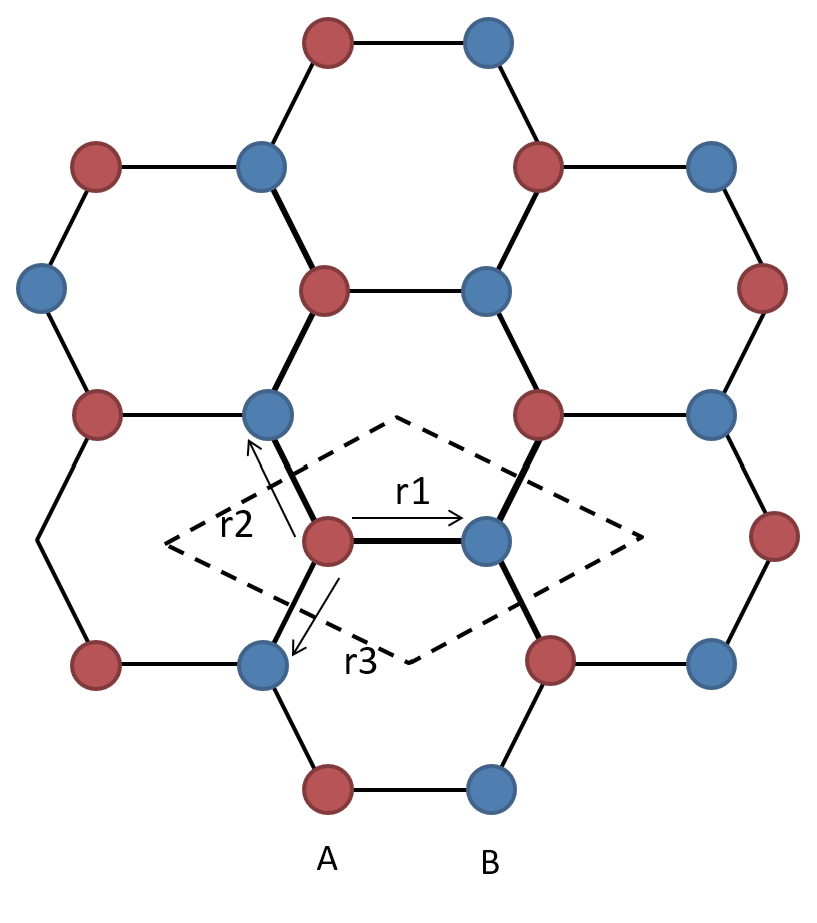
\includegraphics[width=5cm]{graphene.eps}
\end{center}
\label{graphene}
\caption{グラフェンの格子の構造。点線がユニットセルである。$r_1, r_2, r_3$は最近接原子へのベクトルを指す。}
\end{figure}


最近接原子へのベクトル$r_1, r_2, r_3$は炭素の原子間距離をaとすると、それぞれ、
\begin{eqnarray}
r_1=(1,0)a \\
r_2=(-\frac{1}{2}, \frac{\sqrt{3}}{2})a \\
r_3=(-\frac{1}{2}, -\frac{\sqrt{3}}{2})a
\end{eqnarray}
となる。実空間に対するユニットセルの格子ベクトルは
\begin{eqnarray}
a_1=(\frac{3}{2}, -\frac{\sqrt{3}}{2})a \\
a_2=(\frac{3}{2}, \frac{\sqrt{3}}{2})a
\end{eqnarray}
と定義する、この場合逆格子空間での逆格子ベクトルは
\begin{eqnarray}
b_1=(\frac{2\pi}{3a}, -\frac{2\sqrt{3}\pi}{3a}) \\
b_2=(\frac{2\pi}{3a}, \frac{2\sqrt{3}\pi}{3a})
\end{eqnarray}
のようになる。

\begin{figure}[htbp]
\begin{center}
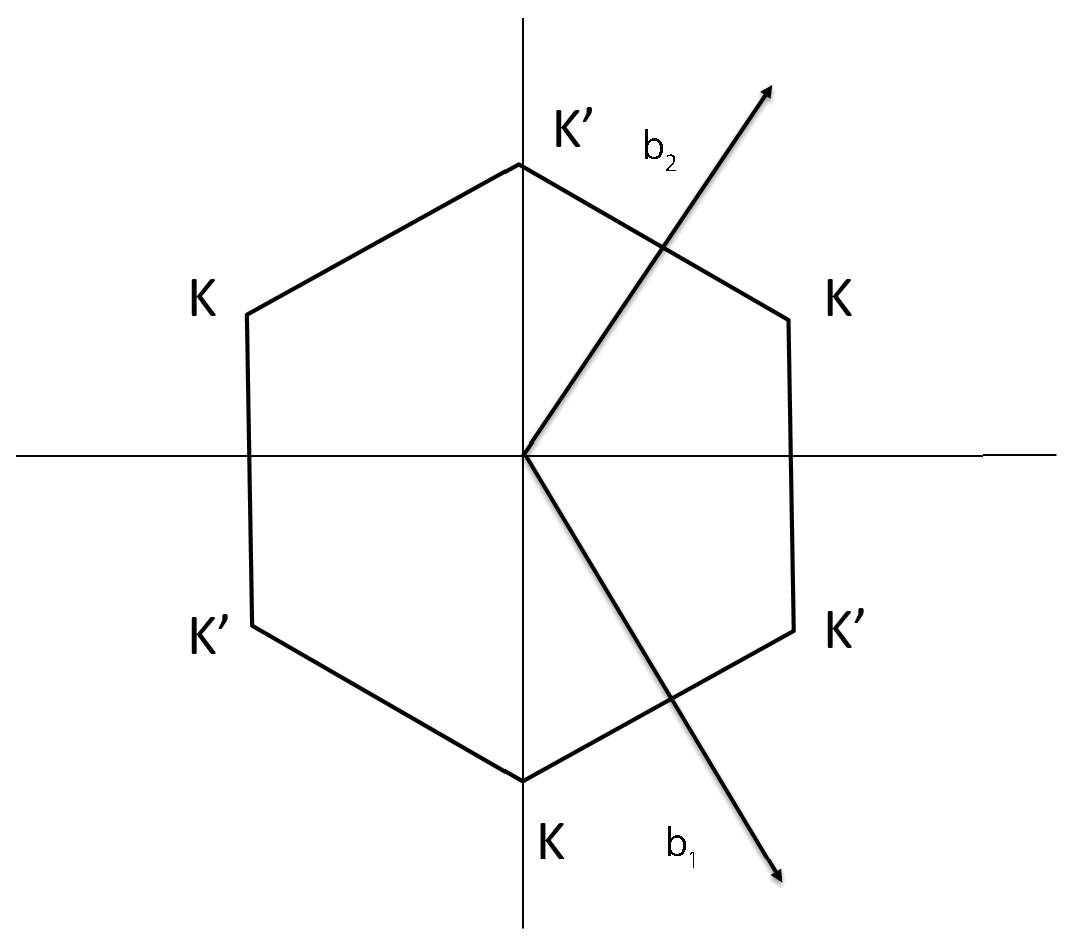
\includegraphics[width=5cm]{Brillouin.eps}
\end{center}
\label{zone}
\caption{ブリルアンゾーンの模式図}
\end{figure}
第一ブリルアンゾーンの6つのコーナーに対応する点は、KとK'の二種類に分類される。
それぞれの座標は
\begin{eqnarray}
K=\frac{4\pi}{3a}(0,-\frac{1}{\sqrt{3}}),\frac{2\pi}{3a}(1,\frac{1}{\sqrt{3}}),\frac{2\pi}{3a}(-1,\frac{1}{\sqrt{3}}) 
\end{eqnarray}

\begin{eqnarray}
K'=\frac{4\pi}{3a}(0,-\frac{1}{\sqrt{3}}),\frac{2\pi}{3a}(1,-\frac{1}{\sqrt{3}}),\frac{2\pi}{3a}(-1,-\frac{1}{\sqrt{3}}) 
\end{eqnarray}
のようになる。

\subsection{グラフェン$\pi$バンドの強束縛模型}
グラフェンにおいて、$\sigma$バンドは面内の強い結合によって深い位置にあり、
伝導を担うフェルミレベル近傍のバンドは$\pi$バンドである。
強束縛模型で電子状態を計算すると、K,K'点で$\pi$バンドと$\pi*$バンドが交差することがわかる。
このことは、簡単な数学的考察で示すことができるので以下に示す。

最近接のみを考えた強束縛模型は、
\begin{eqnarray}
H=\sum_{<i,j>} -t c_A^\dagger(R_i)c_B(R_j) +h.c.
\end{eqnarray}
と書ける。$c_A^\dagger(R_i)$は位置$R_i$のAサイトに電子を生成する演算子であり、
$c_B(R_j)$は位置$R_j$のBサイトの電子を消滅させる演算子である。
$<i,j>$は最近接のペアを取ることに対応している。これらの演算子のフーリエ変換を考えると、
\begin{eqnarray}
c_A^\dagger(R_i)=\sum_{k}c_A^\dagger (k) \exp(-ik\cdot R_i)\\
c_B(R_j)=\sum_{k'}c_B(k') \exp(ik\cdot R_j)
\end{eqnarray}

$R_j$として取りうる値が$R_i+r_1,R_i+r_2,R_i+r_3$であることと、$R_i$に対して和を取る操作で、
k=k'となる項のみが残ることを考えると、
\begin{eqnarray}
H(k)=\sum_{k} f(k) c_A^\dagger(k)c_B(k) +h.c.
\end{eqnarray}
となる。ここで、
\begin{eqnarray}
f(k)=-t(\exp(ik\cdot r_1)+\exp(ik\cdot r_2)+\exp(ik\cdot r_3)) \\
=-t(\exp(ik_x a)+2\exp(\frac{ik_x a}{2})\cos{\frac{\sqrt{3}k_y a}{2}})
\end{eqnarray}
である。行列の形で書くと、
\begin{eqnarray}
H(k)=\left( 
 \begin{array}{cc}
	0 & f(k) \\
	f*(k) & 0
 \end{array}
\right)
\end{eqnarray}
になるため、固有値は
\begin{eqnarray}
\epsilon(k)=\pm |f(k)|
\end{eqnarray}
として得られる。
固有値が0になる波数の条件を考える。
$f(k)$の虚部と実部を考えると、
\begin{eqnarray}
Re f(k)=\cos(k_x a)+2\cos(\frac{k_x a}{2})\cos(\frac{\sqrt{3}k_y a}{2}) =0 \\
Im f(k)=\sin(k_x a)-2\sin(\frac{k_x a}{2})\cos(\frac{\sqrt{3}k_y a}{2}) =0
\end{eqnarray}
を満たす必要がある。
虚部に関する方程式を変形すると、
\begin{eqnarray}
&&\sin(k_x a)-2\sin(\frac{k_x a}{2})\cos(\frac{\sqrt{3}k_y a}{2})\\
&=&2\sin(\frac{k_x
a}{2})\cos(\frac{k_x a}{2})-2\sin(\frac{k_x a}{2})\cos(\frac{\sqrt{3}k_y a}{2})
\\
&=&2\sin(\frac{k_x a}{2})\left\{\cos(\frac{k_x a}{2})-\cos(\frac{\sqrt{3}k_y
a}{2})\right\}
\\
&=&-4\sin(\frac{k_x a}{2})\sin\frac{1}{2}(\frac{k_x a}{2}+\frac{\sqrt{3}k_y
a}{2})\sin\frac{1}{2}(\frac{k_x a}{2}-\frac{\sqrt{3}k_y
a}{2})
\end{eqnarray}
よって、
\begin{eqnarray}
\frac{k_x a}{2}=0 \\
\frac{k_x a}{2}+\frac{\sqrt{3}k_y
a}{2} =0 \\
\frac{k_x a}{2}-\frac{\sqrt{3}k_y
a}{2}=0 
\end{eqnarray}
のいずれかを満たせば良い。$k_x,k_y$の数値については、実部の方程式を合わせて考えることで得られる。
最初の$k_x=0$については、
\begin{eqnarray}
1+2\cos(\frac{\sqrt{3}k_y a}{2})=0
\end{eqnarray}
より
\begin{eqnarray}
k_y=\pm\frac{4\pi}{3\sqrt{3}a}
\end{eqnarray}
が得られる。
二番目の条件からは$k_x=-\sqrt{3}k_y$が得られ、これを実部の方程式に代入することで
\begin{eqnarray}
2\cos(\sqrt{3}k_y a)+1=0
\end{eqnarray}
を得るため、$k_y=\pm \frac{2\pi}{3\sqrt{3}a}$を得る。
同様にして3番目の条件からは、
$k_x=\sqrt{3}k_y$が得られ、同様にして、
$k_y=\pm \frac{2\pi}{3\sqrt{3}a}$を得る。
まとめると、$f(k)=0$を満たす波数kには6つの点があり、それらは
$(k_x,k_y)=(0,\pm\frac{4\pi}{3\sqrt{3}a}), (\frac{2\pi}{3a},\pm \frac{2\pi}{3\sqrt{3}a}),(-\frac{2\pi}{3a},\pm \frac{2\pi}{3\sqrt{3}a})$
である。これらの点がK,K'点に対応することが見て取れる。K点,K'点に分類されるそれぞれ3つの点の間は、逆格子ベクトルの整数倍によって結ぶことができるが、
K,K'点間はそうではないことを付記しておく。

\section{グラフェンとディラックハミルトニアン}
前節で、グラフェンの$\pi$バンドと$\pi*$バンドはK,K'点において、フェルミレベルで交差することを示した。
電子物性は、フェルミレベル近傍の低エネルギーの励起で決まることが多く、低エネルギーでの電子状態を
よく表す有効模型を求めると便利である。
$K,K'$周りでのハミルトニアンを近似する方法として、最も簡単なものが、
\begin{eqnarray}
H(k)=\left( 
 \begin{array}{cc}
	0 & f(k) \\
	f*(k) & 0
 \end{array}
\right)
\end{eqnarray}
を$K,K'$周りでフーリエ展開することである。
\begin{eqnarray}
f(k)\sim f(K)+(k-K)f'(K)
\end{eqnarray}
$q=(k-K), K=(0, -\frac{4\pi}{3\sqrt{3}a})$とすると、
\begin{eqnarray}
\left |\frac{\partial f(k)}{\partial k_x}\right |_{k=K}&=&t \left |ia \exp(ik_x a)-ia\exp(-\frac{ik_x a}{2})\cos(\frac{\sqrt{3}k_y a}{2})\right |_{k=K} \\
&=& -t \frac{3}{2} ia
\end{eqnarray}

\begin{eqnarray}
\left |\frac{\partial f(k)}{\partial k_y}\right |_{k=K}&=&-t \left |\sqrt{3}a\exp(-\frac{ik_x a}{2})\sin(\frac{\sqrt{3}k_y a}{2})\right |_{k=K} \\
&=& t\frac{3}{2} a
\end{eqnarray}
よって、
\begin{eqnarray}
f(k)\sim -t\frac{3}{2}a \left( iq_x+q_y\right)
\end{eqnarray}
を得る。これから直接的に
\begin{eqnarray}
f*(k)\sim -t\frac{3}{2}a \left( -iq_x+q_y\right)
\end{eqnarray}
である。

ここで、座標系全体を-90度回転し、$x\rightarrow-y, y\rightarrow x$としてみよう。
この場合
\begin{eqnarray}
f(k)\sim t\frac{3}{2}a \left( q_x-iq_y\right)
\end{eqnarray}
を得る。これから直接的に
\begin{eqnarray}
f*(k)\sim t\frac{3}{2}a \left( q_x+iq_y\right)
\end{eqnarray}

\begin{eqnarray}
H(k)=\frac{3ta}{2} \left( 
 \begin{array}{cc}
	0 &  q_x-iq_y \\
	q_x+iq_y & 0
 \end{array}
\right)
\end{eqnarray}


上記のハミルトニアンにおいて、$q_x=-i\frac{\partial}{\partial x}$,$q_y=-i\frac{\partial}{\partial y}$
とみなすと、
\begin{eqnarray}
\frac{3ta}{2} \left( 
 \begin{array}{cc}
	0 &  q_x-iq_y \\
	q_x+iq_y & 0
 \end{array}
\right)\left( 
 \begin{array}{c}
	F^K_A(q) \\
	F^K_B(q) 
 \end{array} 
\right)=E 
\left( 
 \begin{array}{c}
	F^K_A(q) \\
	F^K_B(q) 
 \end{array} 
\right)
\end{eqnarray}
という、バンド理論でよく使う、包絡線関数$F^K(q)$に関する有効質量方程式の形を得る。
パウリ行列
\begin{eqnarray}
\sigma_x= \left( 
 \begin{array}{cc}
	0 &  1 \\
	1 & 0
 \end{array}
\right)
\end{eqnarray}

\begin{eqnarray}
\sigma_y= \left( 
 \begin{array}{cc}
	0 &  -i \\
	i & 0
 \end{array}
\right)
\end{eqnarray}

を使うと、

\begin{eqnarray}
\frac{3ta}{2} \left( 
\sigma_x q_x+\sigma_y q_y
\right)F^K(q)=E F^K(q)
\end{eqnarray}
とかけ、これが質量のないDirac方程式(Weyl方程式)と同じ形を持っていることがわかる。
K'点では波数空間の座標の違いによって

\begin{eqnarray}
\frac{3ta}{2} \left( 
\sigma_x q_x-\sigma_y q_y
\right)F^K(q)=E F^K(q)
\end{eqnarray}
のように複素共役の関係にある式が得られる。

形式的には、Weyl方程式と同様の形であるが、パウリ行列は実際のスピンを表しているわけでなく、
波動関数におけるAサイトメインの状態とBサイトメインの状態の重みを表している。
なので、実際のスピンではない量であることを指して、擬スピンと呼ばれる。
(実際のスピンに対しては完全に縮退している)

テイラー展開の最低次までをとると、ディラックハミルトニアンの形が得られることがわかった。
次の次数を含めると、trigonal warpingと呼ばれる、フェルミ面が三角形様に変形していく効果を説明することができる。
2変数関数のテイラー展開に基づくと、2次の項は

\begin{eqnarray}
f^{(2)}(k)\sim \frac{-t}{2} \left \{ \left |\frac{\partial}{\partial k_x}\frac{\partial f(k)}{\partial k_x}\right |_{k=K} q_xq_x 
+2\left |\frac{\partial}{\partial k_x}\frac{\partial f(k)}{\partial k_y}\right |_{k=K} q_xq_y 
+\left |\frac{\partial}{\partial k_y}\frac{\partial f(k)}{\partial k_y}\right |_{k=K} q_yq_y   \right \}
\end{eqnarray}
と書ける。ただし、$\frac{\partial}{\partial k_y}\frac{\partial f(k)}{\partial k_x}=\frac{\partial}{\partial k_x}\frac{\partial f(k)}{\partial k_y}$
であることを用いた。
\begin{eqnarray}
\frac{\partial}{\partial k_x}\frac{\partial f(k)}{\partial k_x}=-a^2 \exp(ik_xa)-\frac{a^2}{2}\exp(-\frac{ik_x a}{2})\cos(\frac{\sqrt{3}k_y a}{2}) \\
\frac{\partial}{\partial k_y}\frac{\partial f(k)}{\partial k_x}=\frac{i\sqrt{3}a^2}{2}\exp(-\frac{ik_x a}{2})\sin(\frac{\sqrt{3}k_y a}{2})\\
\frac{\partial}{\partial k_y}\frac{\partial f(k)}{\partial k_y}=-\frac{3a^2}{2}\exp(-\frac{ik_x a}{2})\cos(\frac{\sqrt{3}k_y a}{2})
\end{eqnarray}

これにk=Kを代入すると
\begin{eqnarray}
f^{(2)}(k)\sim -\frac{3ta^2}{8} (q_x^2-q_y^2 +2iq_xq_y)
\end{eqnarray}
よって
\begin{eqnarray}
f^{(2)}*(k)\sim -\frac{3ta^2}{8} (q_x^2-q_y^2 -2iq_xq_y)
\end{eqnarray}
パウリ行列を用いて、K点周りでの二次の項は、
\begin{eqnarray}
H^{(2)}(k)=-\frac{3ta^2}{8} (\sigma_x(q_x^2-q_y^2) -2\sigma_y q_xq_y)
\end{eqnarray}
と書ける。K'点周りでは
\begin{eqnarray}
H^{(2)}(k)=-\frac{3ta^2}{8} (\sigma_x(q_x^2-q_y^2) +2\sigma_y q_xq_y)
\end{eqnarray}
である。

1次の項と2次の項をもう少しすっきりした形にまとめると、
$\pi=q_x+iq_y, \pi^+=q_x-iq_y$として、
\begin{eqnarray}
H(k)=s\nu  \left( 
 \begin{array}{cc}
	0 &  \pi^+ \\
	\pi & 0
 \end{array}
\right) -\mu \left( 
 \begin{array}{cc}
	0 &  \pi^2 \\
	(\pi^{+})^2 & 0
 \end{array}
\right)
\end{eqnarray}
のようになる。

\begin{figure}[htbp]
\begin{center}
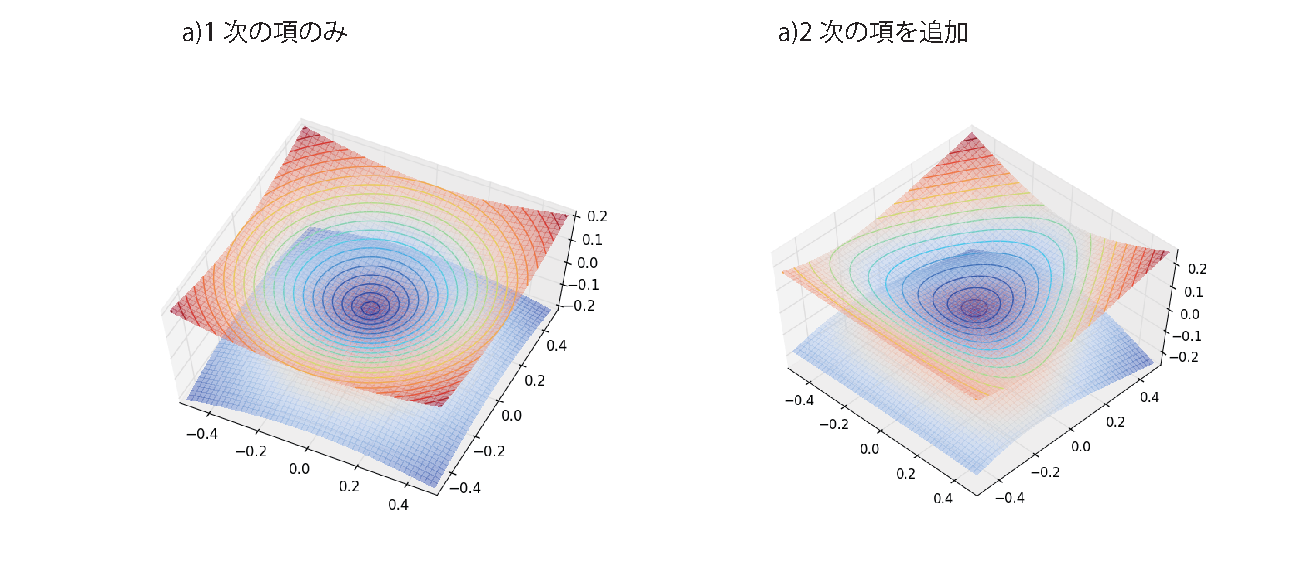
\includegraphics[width=15cm]{trigonalWarping.eps}
\end{center}
\label{trigonal}
\caption{trigonal warpingの効果}
\end{figure}

二次の項の効果を図\ref{trigonal}に示す。
1次の項のみでディラックハミルトニアンの形状になっている場合には、
エネルギー等高面は円形だが、二次の項が加わると、三角形様になっていくのが
わかる。
\section{ディラックハミルトニアンとは}
さて、グラフェンの低エネルギー有効模型が、1次の範囲ではディラックハミルトニアンのそれになることが分かったところで、
ディラックハミルトニアンとは何だったのかを確認しておきたい。
ディラックハミルトニアンは相対論的な量子論における基本手方程式である。
非相対論的な量子論における、シュレーディンガー方程式は、
運動方程式$E=\frac{p^2}{2m}+V$において、
$E \rightarrow i\frac{\partial }{\partial t}, p\rightarrow -i \nabla$
と置き換えることによって
$i\frac{\partial }{\partial t}\psi=\left (-\frac{\nabla^2}{2m}+V \right )\psi$
の形式が得られる。
相対論的な運動方程式は、特殊相対性理論の枠内では
$E^2=p^2+m^2$
となる。(自然単位系として光速度cは1とした)
同様の代入を行うと、
\begin{eqnarray}
\left ( \frac{\partial^2}{\partial t^2}- \frac{\nabla^2}{2m}+m^2\right)\psi =0
\end{eqnarray}
というクライン・ゴルドン方程式を得る。
クライン・ゴルドン方程式は、そのままでは波動関数の確率密度としての解釈が難しいなどの難点が存在する。
これを回避する方法は、ディラックによって生み出された。
ディラックは、シュレディンガー方程式同様の1次微分のみを含む方程式を立てることができれば、
この問題が解決できると考えた。
歴史的には、1次微分のみを含む形式と、それから得られるクライン・ゴルドン方程式と次数が同じ方程式の
係数を比較することでディラック方程式が得られたのだが、
直感的に理解するには、要は因数分解のようなことを行ったとみなすのが簡単である。
もちろん、そのまま因数分解するようなことはうまくいかず、
行列の積を使い、波動関数もベクトル(スピノール)で表すことによってはじめて実現する。

\begin{eqnarray}
(\alpha \cdot p+\beta \cdot m)(\alpha \cdot p+\beta \cdot m)=p^2+m^2
\end{eqnarray}
になればよいので、係数の比較から
\begin{eqnarray}
\alpha^2=\beta^2=1,\\
\alpha_i\alpha_j+\alpha_j\alpha_i=\delta_{ij}, \\
\beta\alpha_i+\alpha_i\beta=0
\end{eqnarray}
が得られる。

まず、簡単なm=0の場合を考えてみよう。(この場合はWeyl方程式と呼ばれる。質量0の粒子が従う方程式である。)
この場合、
\begin{eqnarray}
\alpha_i\alpha_j+\alpha_j\alpha_i=\delta_{ij}
\end{eqnarray}
のみ満たせばよい。
パウリ行列に$\pm 1$をかけたもの$\alpha_i=\pm \sigma_i$はこれを満たす。
ゆえに、正負の符号に対応する2つの解
\begin{eqnarray}
E \psi_L=-\sigma\cdot p \psi_L //
E \psi_R=\sigma\cdot p \psi_R
\end{eqnarray}
が得られる。2つの解を特徴づける量が演算子
$h=\frac{\sigma\cdot p }{|p|}$に対するヘリシティと呼ばれる固有値である。
このことを見るために、平面波解を代入してみる。
$\psi_L$の平面波解は、規格化を無視すると$\psi_L=\exp(-i(Et-p\cdot x))u_L$
のように書くことができる。この場合、Eやpは演算子ではなく、対応する演算子の固有値であるとみなし、
数として扱うことができる。
\begin{eqnarray}
E \psi_L=-\sigma\cdot p \psi_L \rightarrow i\frac{\partial}{\partial t}\phi_L=-i \sigma_i \frac{\partial}{\partial x_i} \psi_L
\end{eqnarray}
として、上記の平面波解を代入すると、改めて
\begin{eqnarray}
E u_L=-\sigma\cdot p u_L
\end{eqnarray}
を得る。ここに$h=\frac{\sigma\cdot p }{|p|}$を両辺から作用させることで
\begin{eqnarray}
\frac{\sigma\cdot p }{|p|}E u_L=-\frac{E^2}{|p|}u_L=-\frac{u_L}{|p|} (p^2+i\sigma(p \times p))
\end{eqnarray}
整理すると
$E^2=p^2$を得る。
エネルギーEが正の解($|p|$)については
\begin{eqnarray}
|p| u_L=-\sigma\cdot p u_L
\end{eqnarray}
となり、これは結局ヘリシティ演算子の固有値が-1であることに対応している(ヘリシティが-1)
一方、エネルギーEが負の解($-|p|$)については
同様の議論により、ヘリシティが1になることがわかる。

まとめると、
$u_L(\psi_L)$は正のエネルギー(粒子)に対してはヘリシティが-1、負のエネルギー(反粒子)に対してはヘリシティが1の解であり
$u_R(\psi_R)$は正のエネルギー(粒子)に対してはヘリシティが1、負のエネルギー(反粒子)に対してはヘリシティが-1の解である。
粒子・反粒子での区別も踏まえたうえで$u_L(\psi_L)$はカイラリティが正の状態、$u_R(\psi_R)$はカイラリティが負の状態であると呼ぶ。
質量0のワイル方程式ではこの2つは独立な解となるが、困ったことにパリティ変換($x\leftrightarrow -x, p\leftrightarrow-p$)を行うと
$\psi_L, \psi_R$が入れ替わるので、パリティ対称性があるような場合(電磁相互作用があるとか)の場合には独立な解ではなくなる。
(Weyl粒子は、ローレンツ対称性を破るので素粒子としては存在しないという例のあれ)
この場合には、$\psi_L, \psi_R$が入り混じったような解が現れる。それを表現するには、方程式を4成分の系に拡大すればよい。
4成分に拡大した場合の方程式は、
\begin{eqnarray}
\Psi=\left( 
 \begin{array}{c}
	\psi_L  \\
	\psi_R
 \end{array}
\right), \\
\alpha=\left( 
 \begin{array}{cc}
	-\sigma &  0 \\
	0 & \sigma
 \end{array}
\right), \\
\beta=\left( 
 \begin{array}{cc}
	0 &  I \\
	I & 0
 \end{array}
\right)
\end{eqnarray}
に対して
$E\Psi=[\alpha \cdot p+\beta m]\Psi$
というものになる。これがいわゆるディラック方程式である。質量項の存在が混合の原因である。
新たな解は、ワイル方程式のようにヘリシティの固有値にはなっていないが
カイラリティ演算子を新たに定義し、その固有状態として分類することができる。
カイラリティ演算子を理解するためには、ガンマ行列をつかってディラック方程式を書き直すと便利である。
ガンマ行列は、ディラック方程式を相対論ぽく(時間を特別扱いしない)書き直すために導入された。


補足)ヘリシティとカイラリティは結局は粒子の運動の向きとスピンがどういう対応関係にあるかに
を表す量で、似ている量といったら似ているが、素粒子の業界では厳密に使い分けられている。
ただ、粒子の運動の向きとスピンの向きに相関があることをカイラルであると表現したり、
エッジ状態になった時に、もともとの意味とよく対応するのかわからないヘリカルエッジ状態・カイラルエッジ状態
という区分が出てきたりするので、非常にややこしい。ヘリカルエッジ状態は二次元トポロジカル絶縁体のように、
上向きスピンと下向きスピンでそれぞれ逆方向に向かうエッジ状態がある状態に相当している。
カイラルエッジ状態は、量子ホール相のエッジ状態に対応していて、どちらか一方向だけに向かうようなエッジ状態が
ある状態に対応している。

\section{ディラック(ワイル)ハミルトニアンの波動関数とBerry位相}
ここで、ディラック(ワイル)ハミルトニアンに戻って、その波動関数を考えてみよう。
(しつこいが、よく出てくるグラフェンでの低エネルギー有効模型は4x4のディラック方程式のサブスペースに対応する
質量0の粒子に対応する2x2のワイルハミルトニアンである。)
簡単のため、$q_x, q_y$のことは、以後$k_x,k_y$と表記する。
\begin{eqnarray}
\gamma \left( 
\sigma_x k_x+\sigma_y k_y
\right)F^K(k)=E F^K(k)
\end{eqnarray}
の固有エネルギーは、$E=\pm \gamma \sqrt{k_x^2+k_y^2}$と求まる。
正のエネルギーが伝導バンドであり、負のエネルギーが価電子バンドである。
このエネルギー固有値を代入して、平面波と振幅部分で波動関数を表記して、振幅の値を求めてやると、
伝導バンドについては
\begin{eqnarray}
F^K(r)=\frac{1}{\sqrt{2}}  \left( 
 \begin{array}{c}
	1  \\
	\frac{k_x+ik_y}{\sqrt{k_x^2+k_y^2}}
 \end{array}
\right) \exp (ikr)
\end{eqnarray}
価電子バンドについては
\begin{eqnarray}
F^K(r)=\frac{1}{\sqrt{2}}  \left( 
 \begin{array}{c}
	-1  \\
	\frac{k_x+ik_y}{\sqrt{k_x^2+k_y^2}}
 \end{array}
\right) \exp (ikr)
\end{eqnarray}
となる。
ここで、波数kを極座標表示してみる。波数ベクトル$k$がx軸となす角度を$\theta_k$とすると、
$k_x=|k|\cos(\theta_k),k_y=|k|\sin(\theta_k) $と表記することができる。
この場合、例えば伝導バンドの波動関数は
\begin{eqnarray}
F^K(r)=\frac{1}{\sqrt{2}}  \left( 
 \begin{array}{c}
	1  \\
	\exp(i\theta_k)
 \end{array}
\right) \exp (ikr)
\end{eqnarray}
価電子バンドは
\begin{eqnarray}
F^K(r)=\frac{1}{\sqrt{2}}  \left( 
 \begin{array}{c}
	-1  \\
	\exp(i\theta_k)
 \end{array}
\right) \exp (ikr)
\end{eqnarray}
と、位相がかかった形で書き表すことができる。
さて、この波動関数で、擬スピンの期待値を求めてみよう。
K点での擬スピンの期待値
$<\sigma>=<<\sigma_x>, <\sigma_y>>$とすると、
伝導バンドについては
\begin{eqnarray}
<\sigma_x>&=&\int \frac{1}{2} (1 \:  \exp(-i\theta_k)) 
\left( 
 \begin{array}{cc}
	0 & 1  \\
	1 & 0
 \end{array}
 \right)
  \left( 
 \begin{array}{c}
	1  \\
	\exp(i\theta_k)
 \end{array}
\right)  \\
 &=& \cos(\theta_k)
\end{eqnarray}

\begin{eqnarray}
<\sigma_y>&=&\int \frac{1}{2} (1 \:  \exp(-i\theta_k)) 
\left( 
 \begin{array}{cc}
	0 & -i  \\
	i & 0
 \end{array}
 \right)
  \left( 
 \begin{array}{c}
	1  \\
	\exp(i\theta_k)
 \end{array}
\right)  \\
 &=& \sin(\theta_k)
\end{eqnarray}


\begin{figure}[hbtp]
\centering
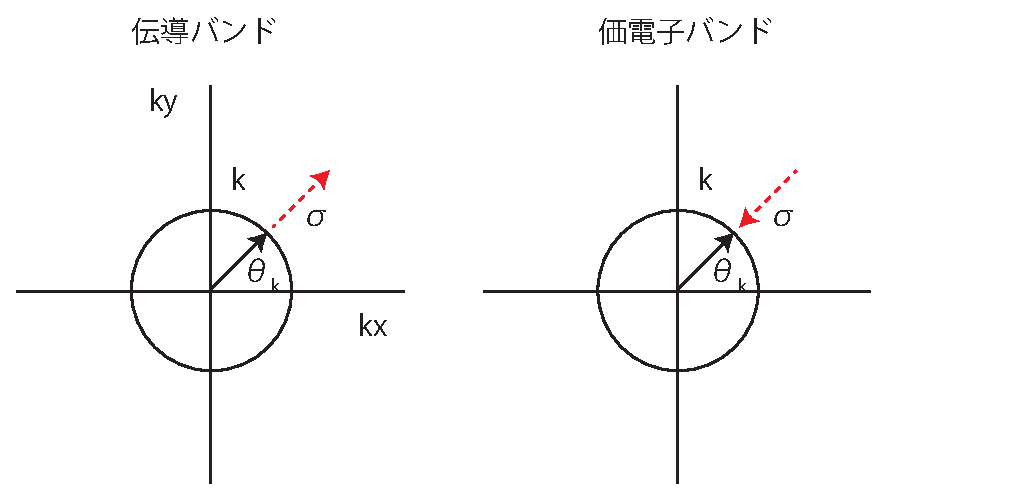
\includegraphics[width=10cm]{psuedoSpin.eps}
\label{pseudo}
\caption{擬スピンと波数の向き}
\end{figure}

よって、伝導バンドについては擬スピンの期待値は$(\cos(\theta_k),\sin(\theta_k))$、
価電子バンドについては$(-\cos(\theta_k),-\sin(\theta_k))$
となることがわかった。

このように、伝導バンドと価電子バンドで擬スピンと波数の向きの対応関係が異なることは
前節でみたようにワイル粒子がヘリシティを持つことに対応している。
(正のエネルギーでヘリシティ1,負のエネルギーでヘリシティ-1なのでカイラリティは正の状態。K'点ではこれが反転してカイラリティが負の状態が現れる。
ただ、グラフェンにおいてはヘリシティとカイラリティが割と混ぜて使われているような感があるのでこの説明があってるかは不安。)

この波動関数を用いて、ベリー位相を計算してみる。
時間t=0からt=Tの間に、波数kが波数空間内で閉曲線を描くようなときに獲得されるベリー位相は

\begin{eqnarray}
\eta=-i \int^T_0 \Bra{F^K(r)} \frac{d}{dt} \Ket{F^K(r)}
\end{eqnarray}
で計算される。波数k、その角度$\theta_k$、位置rがともに時間すると考えると、上記の計算は
\begin{eqnarray}
&&-i \int^T_0 \frac{1}{2} (1 \:  \exp(-i\theta_k))  
\left( 
 \begin{array}{c}
	ir\cdot \frac{\partial k}{\partial t}+ik\cdot  \frac{\partial r}{\partial t} \\
	\exp(i\theta_k)\left \{  i\frac{\partial \theta_k}{\partial t}+ir\cdot\frac{\partial k}{\partial t}+ik\cdot  \frac{\partial r}{\partial t}\right \}
 \end{array}
\right)  \\
&=&-i \int^T_0 \frac{1}{2}\left( i\frac{\partial \theta_k}{\partial t} \right)+ir\cdot\frac{\partial k}{\partial t}+ik\cdot  \frac{\partial r}{\partial t}
\end{eqnarray}
後ろの2つの項は、kが閉曲線を描くことから0になる。よってこの積分値は$\pi$になり、
ベリー位相が通常の0もしくは$2\pi$でなく、特異な$\pi$という値をもつことが示された。


\section{グラフェンにおけるスピン軌道相互作用}
グラフェンのタイトバインディング模型にスピン軌道相互作用の影響を加えたハミルトニアンが
トポロジカル絶縁体のそれと等しくなることを確認する。
グラフェンにおけるスピン軌道相互作用は、$\pi$軌道と$\sigma$軌道の間に
行列要素が生じることによって出てくる。
スピン軌道相互作用や電場による新たな行列要素を摂動として、
$\pi$軌道の有効模型を求めるのには、カノニカル変換を使うと便利である。

SOIならびに電場の影響が加わった場合のグラフェンのタイトバインディングハミルトニアンを
\begin{eqnarray}
H=\left( 
 \begin{array}{cc}
	H_\pi & T \\
	T^\dagger & H_\sigma
 \end{array}
\right)
\end{eqnarray}
で書けるとする。$H_\pi$は$\pi$軌道のハミルトニアンで、スピンも含めると4x4の行列になる。
$H_\pi$は$\pi$軌道のハミルトニアンで$H_\sigma$は$\sigma$軌道のハミルトニアンであり、スピンも含めると12x12の行列である。
カノニカル変換は
\begin{eqnarray}
\tilde{H}=e^{-S} H e^{S}
\end{eqnarray}
で定義される。
Campbell-Baker-Hausdorff公式より
\begin{eqnarray}
\tilde{H}=e^{-S} H e^{S}=H-[S,H]+\frac{1}{2}[S,[S,H]]
\label{CBH}
\end{eqnarray}
と近似できる。1次の項をとり、
\begin{eqnarray}
H-SH+HS
\end{eqnarray}
がブロック対角形で書けることを条件にSを決めると、Sの形状が
\begin{eqnarray}
S=\left( 
 \begin{array}{cc}
	0 & M \\
	-M^\dagger & 0
 \end{array}
\right)
\end{eqnarray}
となり、
\begin{eqnarray}
MH_\sigma -H_\pi M=T \label{M}\\
-M^\dagger H_\pi -H_\sigma M^\dagger=T^\dagger 
\end{eqnarray}
つまり
\begin{eqnarray}
[S, H_0]=H_T 
\end{eqnarray}

\begin{eqnarray}
H_0=\left( 
 \begin{array}{cc}
	H_\pi & 0 \\
	0 & H_\sigma
 \end{array}
\right)
\end{eqnarray}

\begin{eqnarray}
H_T=\left( 
 \begin{array}{cc}
	0 & T \\
	T^\dagger & 0
 \end{array}
\right)
\end{eqnarray}
を満たせばよい。

この関係式を用いて、\ref{CBH}を評価すると、
\begin{eqnarray}
\tilde{H}=H_0-\frac{1}{2}[S, H_T]
\end{eqnarray}
となるため、$\pi$軌道部分の有効ハミルトニアンとしては
\begin{eqnarray}
H_\pi^{eff}=H_\pi-\frac{1}{2}(H_TM^\dagger+MH_T^\dagger)
\end{eqnarray}
を得る。
\ref{M}を用いてMの近似形を定義すると、
\begin{eqnarray}
M=H_TH_\sigma^{-1}+H_\pi MH_\sigma^{-1}~H_TH_\sigma^{-1}
\end{eqnarray}
となり、
\begin{eqnarray}
H_\pi^{eff}=H_\pi-\frac{1}{2}H_T(H_\sigma^{-1\dagger}+H_\sigma^{-1})H_T^\dagger=H_\pi-H_T
H_\sigma^{-1\dagger}H_T^\dagger
\end{eqnarray}
となることがわかる。

有効ハミルトニアンは、$H_\pi, H_\sigma, H_T$が求まればわかることになる。
この方法は\cite{Yao}に従っている。

$\pi$軌道に関するハミルトニアン$H_\pi$,
$\sigma$軌道に関するハミルトニアン、その間を結ぶスピン軌道相互作用によって生じるハミルトニアン$H_T$の形状は $p_x,p_y,
p_z,s$の間のスレーターコスターパラメーターを考えることで求めることができる。
\cite{Yao}は回転行列をつかってサクッと処理しているが、そのやり方だと\cite{Hongki}の結果が再現されない。
その原因は、回転行列を使う方法では、p軌道の位相による飛び移り積分の符号反転が入ってこないからである。

実際に、必要な行列要素を順次計算してみる。スピン軌道相互作用の部分以外は、スピンについて対角成分だけを考えれば良い。
まずAサイトの$p_y$軌道とBサイトの$p_x$軌道の間の飛び移り積分を考えてみる。
Aサイトと最近接Bサイトの間の位置関係を図\ref{NN}のように定義する。
\begin{figure}[hbtp]
\centering
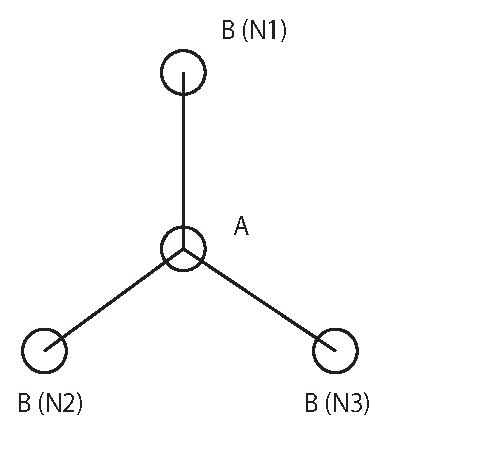
\includegraphics[width=5cm]{nearestNeighbor.eps}
\label{NN}
\caption{最近接原子との関係}
\end{figure}

この時、Aサイトと各最近接原子を結ぶベクトルは
\begin{eqnarray}
N_1=a(0, \frac{1}{\sqrt{3}}) \\
N_2=a(-\frac{1}{2}, -\frac{1}{2\sqrt{3}}) \\
N_3=a(\frac{1}{2}, -\frac{1}{2\sqrt{3}})
\end{eqnarray}
のようになる。
強束縛近似では
\begin{eqnarray}
H_{A\mu, B\mu'}=\sum_{i=1}^3 \exp (i\vec{k}\cdot\vec{N_i})
t_{\mu\mu'}(\vec{N_i})
\end{eqnarray}

であり、今、K点に着目すると
\begin{eqnarray}
\vec{K}\cdot\vec{N_1}=0 \\
\vec{K}\cdot\vec{N_2}=-\frac{2\pi}{3a} \\
\vec{K}\cdot\vec{N_3}=\frac{2\pi}{3a}
\end{eqnarray}

なので、

\begin{eqnarray}
H_{As Bp_x}=tsp_x(\vec{N_1})+\exp (-i\frac{2\pi}{3a})tsp_x(\vec{N_2})+\exp
(i\frac{2\pi}{3a})tsp_x(\vec{N_3}))
\end{eqnarray}
となる。
$tsp_x(\vec{N_1})$はスレーターコスターパラメータ($sp\sigma$)とベクトル$N_1$で決まる方向余弦$e_x$を用いて
\begin{eqnarray}
tsp_x(\vec{N_1})=(sp\sigma)e_x
\end{eqnarray}
と計算できる。
方向余弦はs軌道からpx軌道にホッピングする過程を反映しており、今はx軸から測った角度を使ってcosを計算したものが相当する。
角度の関係は図\ref{ex1}のようになっているので
\begin{figure}[hbtp]
\centering
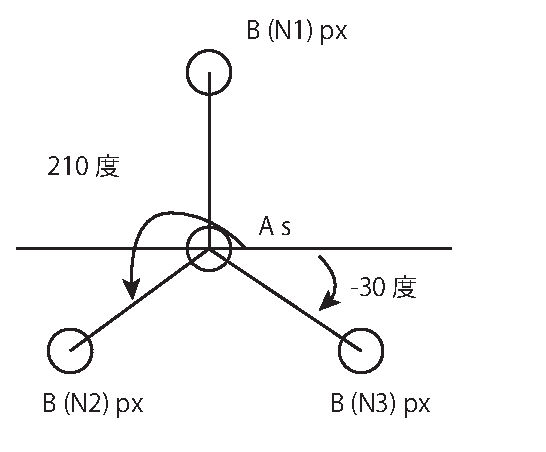
\includegraphics[width=5cm]{hopping1.eps}
\label{ex1}
\caption{方向余弦}
\end{figure}

\begin{eqnarray}
e_x(\vec{N_1})=0 \\
e_x(\vec{N_2})=-\frac{\sqrt{3}}{2} \\
e_x(\vec{N_3})=\frac{\sqrt{3}}{2}
\end{eqnarray}
となる。
故に、

\begin{eqnarray}
H_{As Bp_x}&=&-\frac{\sqrt{3}}{2}(sp\sigma)
\exp(-i\frac{2\pi}{3a})+\frac{\sqrt{3}}{2}(sp\sigma) \exp(i\frac{2\pi}{3a})
\\ \nonumber
&=&\frac{3i}{2}(sp\sigma)
\end{eqnarray}
$\frac{3}{2}(sp\sigma)=\alpha$とすると
\begin{eqnarray}
H_{As Bp_x}=\i\alpha
\end{eqnarray}
となり、\cite{Hongki}での値と一致する。

逆に、Aサイトがpx軌道で、Bサイトがs軌道のパターンを考えてみる。
\begin{eqnarray}
H_{Ap_x Bs}=tp_xs(\vec{N_1})+\exp (-i\frac{2\pi}{3a})tp_xs(\vec{N_2})+\exp
(i\frac{2\pi}{3a})tp_xs(\vec{N_3}))
\end{eqnarray}

スレーターコスターパラメータを使ったと$tpx_s$の評価は、s軌道からpx軌道へのホッピング過程で決まるので、
この場合の方向余弦の定義は\ref{ex2}のようになる。

\begin{figure}[hbtp]
\centering
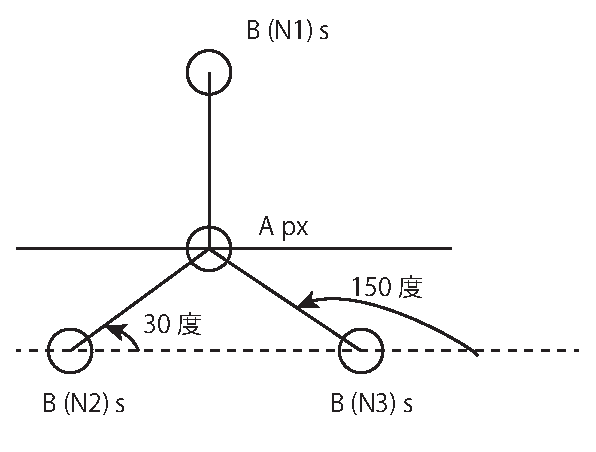
\includegraphics[width=5cm]{hopping2.eps}
\label{ex2}
\caption{方向余弦}
\end{figure}

ゆえに、
\begin{eqnarray}
e_x(\vec{N_1})=0 \\
e_x(\vec{N_2})=\frac{\sqrt{3}}{2} \\
e_x(\vec{N_3})=-\frac{\sqrt{3}}{2}
\end{eqnarray}
のように負号が反転するため、
\begin{eqnarray}
H_{Ap_x Bs}=-\i\alpha
\end{eqnarray}
となる。

同様にして、他のs,p軌道の組み合わせについても計算を行う

\begin{eqnarray}
H_{Ap_x Bp_y}=tp_xp_y(\vec{N_1})+\exp (-i\frac{2\pi}{3a})tp_xp_y(\vec{N_2})+\exp
(i\frac{2\pi}{3a})tp_xp_y(\vec{N_3}))
\end{eqnarray}

\begin{eqnarray}
tp_xp_y(\vec{N})=(pp\sigma)e_xe_y -(pp\pi)e_xe_y
\end{eqnarray}

\begin{eqnarray}
e_x(\vec{N_1})=0, e_y(\vec{N_1})=1 \\
e_x(\vec{N_2})=-\frac{\sqrt{3}}{2}, e_y(\vec{N_2})=-\frac{1}{2} \\
e_x(\vec{N_3})=\frac{\sqrt{3}}{2}, e_y(\vec{N_2})=-\frac{1}{2}
\end{eqnarray}
なので、
\begin{eqnarray}
H_{Ap_x Bp_y}&=&\frac{\sqrt{3}}{4}\{ (pp\sigma)-(pp\pi)\}e^{
-i\frac{2\pi}{3a}}-\frac{\sqrt{3}}{4}\{ (pp\sigma)-(pp\pi)\}e^{i\frac{2\pi}{3a}}
\\ \nonumber
&=& -\frac{3i}{4}\{ (pp\sigma)-(pp\pi)\}
\end{eqnarray}

$\frac{3}{4}\{ (pp\sigma)-(pp\pi)\}=\beta$とすると
$H_{Ap_x Bp_y}=-i\beta$


\begin{eqnarray}
H_{Ap_y Bp_x}=tp_yp_x(\vec{N_1})+\exp (-i\frac{2\pi}{3a})tp_yp_x(\vec{N_2})+\exp
(i\frac{2\pi}{3a})tp_yp_x(\vec{N_3}))
\end{eqnarray}

\begin{eqnarray}
tp_yp_x(\vec{N})=(pp\sigma)e_xe_y -(pp\pi)e_xe_y
\end{eqnarray}
の方向余弦の定義が、前述のように変化し
\begin{eqnarray}
e_x(\vec{N_1})=0, e_y(\vec{N_1})=-1 \\
e_x(\vec{N_2})=\frac{\sqrt{3}}{2}, e_y(\vec{N_2})=\frac{1}{2} \\
e_x(\vec{N_3})=-\frac{\sqrt{3}}{2}, e_y(\vec{N_2})=\frac{1}{2}
\end{eqnarray}
なので、
\begin{eqnarray}
H_{Ap_x Bp_y}&=&\frac{\sqrt{3}}{4}\{ (pp\sigma)-(pp\pi)\}e^{
-i\frac{2\pi}{3a}}-\frac{\sqrt{3}}{4}\{ (pp\sigma)-(pp\pi)\}e^{i\frac{2\pi}{3a}}
\\ \nonumber
&=& -\frac{3i}{4}\{ (pp\sigma)-(pp\pi)\}
\end{eqnarray}
よって
$H_{Ap_yBp_x}=-i\beta$

また、
\begin{eqnarray}
H_{Ap_x Bp_x}=tp_xp_x(\vec{N_1})+\exp (-i\frac{2\pi}{3a})tp_xp_x(\vec{N_2})+\exp
(i\frac{2\pi}{3a})tp_xp_x(\vec{N_3}))
\end{eqnarray}
ここで、
\begin{eqnarray}
tp_xp_x(\vec{N})=(pp\sigma)e^2_x -(pp\pi)(1-e^2_x)
\end{eqnarray}
である。前回計算したように
\begin{eqnarray}
e_x(\vec{N_1})=0, e_y(\vec{N_1})=1 \\
e_x(\vec{N_2})=-\frac{\sqrt{3}}{2}, e_y(\vec{N_2})=-\frac{1}{2} \\
e_x(\vec{N_3})=\frac{\sqrt{3}}{2}, e_y(\vec{N_2})=-\frac{1}{2}
\end{eqnarray}
なので、
\begin{eqnarray}
H_{Ap_x Bp_x}&=&(pp\pi)+\{ \frac{3}{4}(pp\sigma)+ \frac{1}{4}(pp\pi)\}e^{
-i\frac{2\pi}{3a}}+\{\frac{3}{4}
(pp\sigma)+\frac{1}{4}(pp\pi)\}e^{i\frac{2\pi}{3a}}  \nonumber \\
&=& -\frac{3}{4}\{ (pp\sigma)-(pp\pi)\}
\end{eqnarray}

ゆえに
$H_{Ap_x Bp_x}=-\beta$


さらに、
\begin{eqnarray}
H_{Ap_y Bp_y}=tp_yp_y(\vec{N_1})+\exp (-i\frac{2\pi}{3a})tp_yp_y(\vec{N_2})+\exp
(i\frac{2\pi}{3a})tp_yp_y(\vec{N_3}))
\end{eqnarray}
ここで、
\begin{eqnarray}
tp_yp_y(\vec{N})=(pp\sigma)e^2_y -(pp\pi)(1-e^2_y)
\end{eqnarray}
である。前回の方向余弦の計算を用いると
\begin{eqnarray}
H_{Ap_y Bp_y}&=&(pp\sigma)+\{ \frac{1}{4}(pp\sigma)+ \frac{3}{4}(pp\pi)\}e^{
-i\frac{2\pi}{3a}}+\{\frac{1}{4}
(pp\sigma)+\frac{3}{4}(pp\pi)\}e^{i\frac{2\pi}{3a}}  \nonumber \\
&=& \frac{3}{4}\{ (pp\sigma)-(pp\pi)\}
\end{eqnarray}

ゆえに
$H_{Ap_y Bp_y}=\beta$


最後に、
\begin{eqnarray}
H_{As Bp_y}=tsp_y(\vec{N_1})+\exp (-i\frac{2\pi}{3a})tsp_y(\vec{N_2})+\exp
(i\frac{2\pi}{3a})tsp_y(\vec{N_3}))
\end{eqnarray}
ここで、
\begin{eqnarray}
tsp_y(\vec{N})=(sp\sigma)e_y 
\end{eqnarray}
である。前回の方向余弦の計算を用いると
\begin{eqnarray}
H_{As Bp_y}&=&(sp\sigma)-\frac{1}{2}(sp\sigma)e^{
-i\frac{2\pi}{3a}}-\frac{1}{2}
(sp\sigma)e^{i\frac{2\pi}{3a}}  \nonumber \\
&=& \frac{3}{2}(sp\sigma)
\end{eqnarray}

ゆえに
$H_{As Bp_y}=\alpha$

同様にして
\begin{eqnarray}
H_{Ap_y Bs}&=&-(sp\sigma)+\frac{1}{2}(sp\sigma)e^{
-i\frac{2\pi}{3a}}+\frac{1}{2}
(sp\sigma)e^{i\frac{2\pi}{3a}}  \nonumber \\
&=& -\frac{3}{2}(sp\sigma) =-\alpha
\end{eqnarray}

これらの関係式は\cite{Hongki}と一致している。
得られたABサイト間をつなぐハミルトニアンの行列要素をAs, Apx, Apy, Apz, Bs, Bpx, Bpy, Bpzの順で並べた6つの基底を使って
行列の形で表現すると、以下のようになる。ここでsはp軌道の準位を基準にして測ったs軌道のエネルギーである。


\begin{doublespace}
\noindent\(\pmb{\left(
\begin{array}{cccccc}
 s & 0 & 0 & 0 & i \alpha  & \alpha  \\
 0 & 0 & 0 & -i \alpha  & -\beta  & -i \beta  \\
 0 & 0 & 0 & -\alpha  & -i \beta  & \beta  \\
 0 & i \alpha  & -\alpha  & s & 0 & 0 \\
 -i \alpha  & -\beta  & i \beta  & 0 & 0 & 0 \\
 \alpha  & i \beta  & \beta  & 0 & 0 & 0 \\
\end{array}
\right)}\)
\end{doublespace}

次に必要となるのが、スピン軌道相互作用によって、p軌道間をつなぐ行列要素の計算である。
スピン軌道相互作用は局所的であり、同一サイトのみに働くと考える。
この場合
\begin{eqnarray}
H_{soi}=\xi \vec{l}\cdot\vec{s} =\xi \{\frac{l^+\cdot s^- + l^-\cdot s^+}{2}
+l^z \cdot s^z
\}
\end{eqnarray}
のようにハミルトニアンを近似できる。
この行列要素を計算するためには、px, pyは球面調和関数の線形結合に焼き直したほうがよい。

\begin{eqnarray}
p_x=-\frac{1}{\sqrt{2}} (Y_{11}-Y_{1-1}) \\
p_y=-\frac{1}{\sqrt{2}i} (Y_{11}+Y_{1-1})
\end{eqnarray}
であるから、$p_z=Y_{10}$であることを考えると
\begin{eqnarray}
\Bra{p_z \downarrow} H_{soi}\Ket{p_x \uparrow} =\frac{1}{2\sqrt{2}}\Bra{Y_{10}
\downarrow} H_{soi} \Ket{Y_{1-1} \uparrow} =\frac{\xi}{2}
\end{eqnarray}

\begin{eqnarray}
\Bra{p_z \uparrow} H_{soi} \Ket{p_x \downarrow} =\frac{1}{2\sqrt{2}} \Bra{Y_{10}
\uparrow} H_{soi} \Ket{Y_{11} \downarrow} =-\frac{\xi}{2}
\end{eqnarray}

\begin{eqnarray}
\Bra{p_z \downarrow} H_{soi}\Ket{p_y \uparrow} =\frac{i}{2\sqrt{2}}\Bra{Y_{10}
\downarrow} H_{soi}\Ket{Y_{1-1} \uparrow} =\frac{i\xi}{2}
\end{eqnarray}

\begin{eqnarray}
\Bra{p_z \uparrow} H_{soi}\Ket{p_y \downarrow} =\frac{i}{2\sqrt{2}}\Bra{Y_{10}
\uparrow} H_{soi}\Ket{Y_{11} \downarrow} =\frac{i\xi}{2}
\end{eqnarray}

よって、各行がAまたはBサイトの$p_z \uparrow$, $p_z \downarrow$ 各列が $s \uparrow$, $s
\downarrow, p_x \uparrow$, $p_x \downarrow, p_y \uparrow$, $p_y \downarrow$
に対応する2x4の行列は

\begin{doublespace}
\noindent\(\left(
\begin{array}{cccccccccccc}
 0 & 0 & 0 & -\frac{1}{2} & 0 & \frac{i}{2} & 0 & 0 & 0 & 0 & 0 & 0 \\
 0 & 0 & \frac{1}{2} & 0 & \frac{i}{2} & 0 & 0 & 0 & 0 & 0 & 0 & 0 \\
 0 & 0 & 0 & 0 & 0 & 0 & 0 & 0 & 0 & -\frac{1}{2} & 0 & \frac{i}{2} \\
 0 & 0 & 0 & 0 & 0 & 0 & 0 & 0 & \frac{1}{2} & 0 & \frac{i}{2} & 0 \\
\end{array}
\right)\)
\end{doublespace}

にスピン軌道相互作用定数$\xi$をかけたものになる。

前述のσ軌道部分のハミルトニアンをスピンも含む形に拡張し、更にA,Bサイト同士の対角項も加えたものが$H_\sigma$であり、
それは以下のような形状を取る。

\begin{doublespace}
\noindent\(\left(
\begin{array}{cccccccccccc}
 s & 0 & 0 & 0 & 0 & 0 & 0 & 0 & i \alpha  & 0 & \alpha  & 0 \\
 0 & s & 0 & 0 & 0 & 0 & 0 & 0 & 0 & i \alpha  & 0 & \alpha  \\
 0 & 0 & 0 & 0 & 0 & 0 & -i \alpha  & 0 & -\beta  & 0 & -i \beta  & 0 \\
 0 & 0 & 0 & 0 & 0 & 0 & 0 & -i \alpha  & 0 & -\beta  & 0 & -i \beta  \\
 0 & 0 & 0 & 0 & 0 & 0 & -\alpha  & 0 & -i \beta  & 0 & \beta  & 0 \\
 0 & 0 & 0 & 0 & 0 & 0 & 0 & -\alpha  & 0 & -i \beta  & 0 & \beta  \\
 0 & 0 & i \alpha  & 0 & -\alpha  & 0 & s & 0 & 0 & 0 & 0 & 0 \\
 0 & 0 & 0 & i \alpha  & 0 & -\alpha  & 0 & s & 0 & 0 & 0 & 0 \\
 -i \alpha  & 0 & -\beta  & 0 & i \beta  & 0 & 0 & 0 & 0 & 0 & 0 & 0 \\
 0 & -i \alpha  & 0 & -\beta  & 0 & i \beta  & 0 & 0 & 0 & 0 & 0 & 0 \\
 \alpha  & 0 & i \beta  & 0 & \beta  & 0 & 0 & 0 & 0 & 0 & 0 & 0 \\
 0 & \alpha  & 0 & i \beta  & 0 & \beta  & 0 & 0 & 0 & 0 & 0 & 0 \\
\end{array}
\right)\)
\end{doublespace}

スピン軌道相互作用による効果を表す$H_T$は、ABサイト双方も含んだ形に拡張すると

\begin{doublespace}
\noindent\(\left(
\begin{array}{cccccccccccc}
 0 & 0 & 0 & -\frac{1}{2} & 0 & \frac{i}{2} & 0 & 0 & 0 & 0 & 0 & 0 \\
 0 & 0 & \frac{1}{2} & 0 & \frac{i}{2} & 0 & 0 & 0 & 0 & 0 & 0 & 0 \\
 0 & 0 & 0 & 0 & 0 & 0 & 0 & 0 & 0 & -\frac{1}{2} & 0 & \frac{i}{2} \\
 0 & 0 & 0 & 0 & 0 & 0 & 0 & 0 & \frac{1}{2} & 0 & \frac{i}{2} & 0 \\
\end{array}
\right)\)
\end{doublespace}
という行列全体にスピン軌道相互作用定数$\xi$をかけたものになる
これらの行列を使って$-H_T
H_\sigma^{-1\dagger}H_T^\dagger$を計算すると


\begin{doublespace}
\noindent\(\left(
\begin{array}{cccc}
 0 & 0 & 0 & 0 \\
 0 & \frac{s \xi^2}{4 \alpha ^2} & 0 & 0 \\
 0 & 0 & \frac{s \xi^2}{4 \alpha ^2} & 0 \\
 0 & 0 & 0 & 0 \\
\end{array}
\right)\)
\end{doublespace}

が出て来る。これをパウリ行列を使って書き直すと
\begin{eqnarray}
H_{eff}=-H_T
H_\sigma^{-1\dagger}H_T^\dagger = -\lambda_{SO}+\lambda_{SO} \sigma_z s_z
\end{eqnarray}
となる。ただし、$2\lambda_{SO}=\frac{s}{4 \alpha
^2}=\frac{|s|
\xi^2}{9(sp\sigma)^2}$である。ここまでの計算はK
に注目してきたが、K'でも同様の計算を行うことができる。
ただし、この場合、K'の波数がKと負号が反転していることを反映して
得られる有効相互作用にも負号が含まれてくる。
K,K'のバレー種別を擬スピン$\tau_z$で表すと、これは更に
\begin{eqnarray}
H_eff= -\lambda_{SO}+\lambda_{SO} \sigma_z \tau_z s_z
\end{eqnarray}
となる。ただし、ここでパウリ行列や擬スピン、スピンの積とは、テンソル積(クロネッカー積)であることに注意する。
この形は、Kane-Mele模型\cite{Kane1}で導入されたスピン軌道相互作用の効果と同様の構造を持っていることが分かる。

さらにこの方法を垂直方向の電場が加わった場合のラシュバ項の導出へと拡張することもできる。
電場が加わったときに生じる追加の項は、A, B各サイトにおけるシュタルク効果に対応するものである。
s-p軌道間に生じるシュタルク効果の行列要素を$eEz_0$とおくと、垂直電場の効果は$H_T$を

\begin{doublespace}
\noindent\(\left(
\begin{array}{cccccccccccc}
 \text{e$Ez_0$} & 0 & 0 & -\frac{1}{2} & 0 & \frac{i}{2} & 0 & 0 & 0 & 0 & 0 & 0
 \\
 0 & \text{e$Ez_0$} & \frac{1}{2} & 0 & \frac{i}{2} & 0 & 0 & 0 & 0 & 0 & 0 & 0
 \\
 0 & 0 & 0 & 0 & 0 & 0 & \text{e$Ez_0$} & 0 & 0 & -\frac{1}{2} & 0 & \frac{i}{2}
 \\
 0 & 0 & 0 & 0 & 0 & 0 & 0 & \text{e$Ez_0$} & \frac{1}{2} & 0 & \frac{i}{2} & 0
 \\
\end{array}
\right)\)
\end{doublespace}

と拡張すればよい。

\begin{doublespace}
\noindent\(\pmb{\left(
\begin{array}{cccc}
 0 & 0 & 0 & 0 \\
 0 & \frac{s}{4 \alpha ^2} & \frac{i \text{e$Ez_0$}}{ \alpha } & 0 \\
 0 & -\frac{i \text{e$Ez_0$}}{ \alpha } & \frac{s}{4 \alpha ^2} & 0 \\
 0 & 0 & 0 & 0 \\
\end{array}
\right)}\)
\end{doublespace}

これをパウリ行列を使って書き直すと
\begin{eqnarray}
H_{eff}=-H_T
H_\sigma^{-1\dagger}H_T^\dagger = -\lambda_{SO}+\lambda_{SO} \sigma_z
s_z+\lambda_{R} (\sigma_x s_y -\sigma_{y} s_x)
\end{eqnarray}
ここで、$\lambda_R=\frac{eEz_0 \xi}{3(sp\sigma)}$である。
バレー擬スピンも含めて書くと、
\begin{eqnarray}
H_{eff}= -\lambda_{SO}+\lambda_{SO} \sigma_z \tau_z s_z+\lambda_{R} (\sigma_x
\tau_z s_y -\sigma_{y} s_x)
\end{eqnarray}
となる。

\section{磁場下の格子模型}
前節で一応、スピン軌道相互作用がもたらす、グラフェンのようなハニカム格子系で、ディラック分散を作る$\pi$バンドと
他のp軌道や、それらのp軌道とs軌道との混ざり合いを有効模型として$\pi$バンドに押し込むと、
連続極限における
\begin{eqnarray}
H_{eff}=  v_F (\sigma_x\tau_y q_x + \sigma_y q_y)+\lambda_{SO} \sigma_z \tau_z
s_z+\lambda_{R} (\sigma_x \tau_z s_y -\sigma_{y} s_x)
\end{eqnarray}
が出てくることは納得できる。
ただ、よくわからないのが、エッジ状態やらブリルアンゾーン全域でのバンドを考えて、
Z2の議論をするために格子模型にしたときの
\begin{eqnarray}
H=\Sigma_{<ij>\alpha} tc_{i\alpha}^\dagger c_{j\alpha}+\Sigma_{<<ij>>\alpha
\beta} it_2 \nu_{ij} s_\alpha\beta ^z c_{i\alpha}^\dagger c_{j\alpha}
\end{eqnarray}
の第二項である。なぜに第二近接のホッピングを考えるのか?あとホッピング方向で決まる$\nu_{ij}$ってどこから出てくるのか?
これの元になっているのはHaldaneの模型であるが、それに遡っても上記の問題は解決しない。

これらのHaldane模型とかの格子模型を理解するためには、スピン軌道相互作用の効果を露わに考えるよりは、
まず、格子模型における磁場効果の取り入れ方から学ぶほうが理解しやすい。

\subsection{パイエルス位相}
量子力学における磁場の効果は一般的に、
電子の運動量$p=-i\hbar \nabla$を$p+eA/c$に置き換えてやることで取り入れられることが知られている。
(eの定義が正か負か要注意。ここでは正で定義する)。
空間のある場所には磁場がかかっている(磁束、Aのrotationがある)が、その他の領域には磁場がかかっていないような状態を考える。
磁場がかかっていない領域を運動する電子の波動関数は、磁場がそもそも無い時の波動関数$\psi^0(x)$をつかって
\begin{eqnarray}
\psi(x)=\psi^0(x) \exp \left[\frac{ie}{\hbar c}\int^s(x) A(x')dx'\right]
\end{eqnarray}

となることが知られている。$s(x)$は線積分の経路を示す。端的に言うと、ベクトルポテンシャルの影響は
波動関数の位相変化として拾われる。
この波動関数の形や位相の値自体は、どのようなゲージを取るかで任意性がある。しかし、ベリー位相と同じで、
積分経路が閉じた場合には、
\begin{eqnarray}
-\frac{e}{h}\oint A(x')dx' =-2\pi \frac{\Phi}{\Phi_0}
\end{eqnarray}
の閉曲線で囲まれる範囲を貫く磁束$\Phi$で決まる位相(アハラノフ・ボーム位相)が一意に決まる。

これらの原則を使って、磁場下の格子模型をタイトバインディング模型で表したときに、
位相の情報をどうやってタイトバインディング模型に乗せれば良いのかを考える。
タイトバインディング模型に乗っかってくる位相のことをパイエルス位相と呼ぶ。
簡単な例として、二次元の正方格子を考える。格子定数は簡単のため1とする。

二次元正方格子のタイトバインディング模型は、一般的に
\begin{eqnarray}
H_0=-J\sum_{m,n} \left(a_{m+1,n}^\dagger a_{m,n}+a_{m,n+1}^\dagger a_{m,n}+
h.c.\right)
\end{eqnarray}
のように書ける。ここに磁場$B=\nabla\times A$が加わると、前の議論から、電子は飛び移る経路に応じて
位相を獲得すると予想できる。格子点(m,n)からx方向もしくはy方向に+1移動する時に獲得する位相(パイエルス位相)を
\begin{eqnarray}
\phi_{m,n}^i=-e\frac{A_{m,n}^i}{\hbar} 
\end{eqnarray}
(i=x,y)であると単純に考えて、このベクトルポテンシャルが加わった時のタイトバインディング模型は
\begin{eqnarray}
H=-J\sum_{m,n} \left(e^{i\phi_{m,n}^x}a_{m+1,n}^\dagger
a_{m,n}+e^{i\phi_{m,n}^y}a_{m,n+1}^\dagger a_{m,n}+ h.c.\right)
\label{H}
\end{eqnarray}

ユニットセルを貫く磁束とこれらの位相との間の関係は、正方格子の中の正方形の周りを一周するホッピング経路が図\ref{sq}
のようになることから求められる。(経路が逆転すると負号が逆になっていることに注意。)

\begin{figure}[hbtp]
\centering
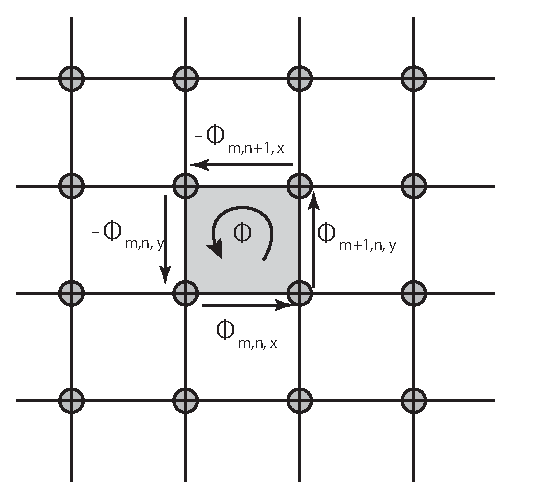
\includegraphics[width=5cm]{square-lattice.eps}
\label{sq}
\caption{正方格子でのユニットセルあたりの磁束}
\end{figure}

\begin{eqnarray}
\Phi=\frac{1}{2\pi}\left(\phi_{m,n}^x+\phi_{m+1,n}^y-\phi_{m,n+1}^x-\phi_{m,n}^y
\right)
\end{eqnarray}

こう見ると、なんとなくこれで磁場下のタイトバインディング模型が得られたように思えるが、一つ問題がある。
それは、並進対称性をどうやって定義するかである。

元々のゼロ磁場でのタイトバインディング模型は
\begin{eqnarray}
T_x^0=\sum_{m,n}a_{m+1,n}^\dagger
a_{m,n}, T_y^0=\sum_{m,n}a_{m,n+1}^\dagger
a_{m,n} 
\end{eqnarray}
という風に並進対称演算子を定義したときに、
\begin{eqnarray}
[H_0,T_x^0]=[H_0,T_y^0]=0
\end{eqnarray}
を満たす。しかし、磁場がある時にこれを直接拡張すると
\begin{eqnarray}
T_x=\sum_{m,n} e^{i\psi_{m,n}^x}a_{m+1,n}^\dagger
a_{m,n}, T_y=\sum_{m,n}e^{i\psi_{m,n}^y}a_{m,n+1}^\dagger
a_{m,n} 
\end{eqnarray}
は、ハミルトニアン\ref{H}とは交換しない。
なぜならば、$[T_x, T_y] \neq 0$でお互いに交換しないからである。
これは、
\begin{eqnarray}
T_x T_y \Ket{\psi_{ij}}&=&T_x T_y c_{ij}^\dagger \Ket{0} \nonumber \\
&=& T_x \sum_{m,n} c_{m,n+1}^\dagger c_{m,n} e^{i\phi_{m,n}^y}c_{i,j}^\dagger
\Ket{0} \nonumber \\
&=& T_x e^{i\phi_{i,j}^y} c_{i,j+1}^\dagger \Ket{0} \nonumber \\
&=& e^{i\phi_{i,j}^y} \sum_{m,n}e^{i\psi_{m,n}^x} c_{m+1,n}^\dagger c_{m,n}
c_{i,j+1}^\dagger \Ket{0} \nonumber \\
&=& e^{i \left( \phi_{i,j}^y+ \phi_{i, j+1}^x\right)}  c_{i+1,j+1}^\dagger
\Ket{0}
\end{eqnarray}
と、同様にして得られる
\begin{eqnarray}
T_y T_x \Ket{\psi_{ij}}
= e^{i \left( \phi_{i+1,j}^y+ \phi_{i, j}^x\right)}  c_{i+1,j+1}^\dagger
\Ket{0}
\end{eqnarray}
を比較すれば理解できる。

そこで、磁場に対する並進対称演算子の形を、ゲージ変換を加えたもので定義する。

\begin{eqnarray}
T_x^M=\sum_{m,n} e^{i\theta_{m,n}^x}a_{m+1,n}^\dagger
a_{m,n}, \nonumber \\
T_y^M=\sum_{m,n}e^{i\theta_{m,n}^y}a_{m,n+1}^\dagger
a_{m,n} 
\end{eqnarray}

ゲージ変換を加えたもの磁場の効果を含めた上での並進演算子がハミルトニアンと交換する条件を導く。
\begin{eqnarray}
[T_x,T_x^M]=[T_x^M, T_y]=[T_y^M, T_x]=[T_y^M, T_y]=0
\end{eqnarray}
を満たす必要がある。
まず$[T_x,T_x^M]$を計算してみる。
\begin{eqnarray}
[T_x,T_x^M]=[\sum_{mn}c_{m+1,n}^\dagger c_{m,n}e^{i\phi_{m,n}^x},
\sum_{m'n'}c_{m'+1,n'}^\dagger c_{m',n'}e^{i\theta_{m',n'}^x}]
\end{eqnarray}
この交換関係を解釈するために、

\begin{eqnarray}
\sum_{m',n', m,n}c_{m'+1,n'}^\dagger
c_{m',n'}e^{i\theta_{m',n'}^x}c_{m+1,n}^\dagger c_{m,n}e^{i\phi_{m,n}^x}
\end{eqnarray}
のオペレータの順序を交換することを考える

\begin{eqnarray}
&&\sum_{m',n', m,n}c_{m'+1,n'}^\dagger
c_{m',n'}e^{i\theta_{m',n'}^x}c_{m+1,n}^\dagger c_{m,n}e^{i\phi_{m,n}^x}
\nonumber \\
&=&\delta_{m',m+1}\delta_{n',n} \sum_{m',n', m,n} c_{m'+1, n'} c_{m,n}
e^{i\theta_{m',n'}^x} e^{i\phi_{m,n}^x} \nonumber \\
&-&\sum_{m',n',
m,n}c_{m'+1,n'}^\dagger c_{m+1,n}^\dagger
c_{m',n'} c_{m,n} e^{i\theta_{m',n'}^x} e^{i\phi_{m,n}^x} \nonumber \\
&=&\sum_{m,n} c_{m+2, n} c_{m,n}
e^{i\theta_{m+1,n}^x} e^{i\phi_{m,n}^x} \nonumber \\
&+&\sum_{m',n',
m,n} c_{m+1,n}^\dagger c_{m'+1,n'}^\dagger 
c_{m',n'} c_{m,n} e^{i\theta_{m',n'}^x} e^{i\phi_{m,n}^x} \nonumber \\
&=&\sum_{m,n} c_{m+2, n} c_{m,n}
e^{i\theta_{m+1,n}^x} e^{i\phi_{m,n}^x} \nonumber \\
&-& \delta_{m'+1,m} \delta_{n',n} \sum_{m',n',
m,n} c_{m+1,n}^\dagger c_{m',n'} e^{i\theta_{m',n'}^x} e^{i\phi_{m,n}^x}  \nonumber \\
&+& \sum_{m',n',
m,n} c_{m+1,n}^\dagger c_{m,n} c_{m'+1,n'}^\dagger 
c_{m',n'} e^{i\theta_{m',n'}^x} e^{i\phi_{m,n}^x} \nonumber \\
&=&\sum_{m,n} c_{m+2, n} c_{m,n}
e^{i\theta_{m+1,n}^x} e^{i\phi_{m,n}^x} \nonumber \\
&-& \sum_{m,n} c_{m+1,n}^\dagger c_{m-1,n} e^{i\theta_{m-1,n}^x}
e^{i\phi_{m,n}^x}  \nonumber \\
&+& \sum_{m',n',
m,n} c_{m+1,n}^\dagger c_{m,n} c_{m'+1,n'}^\dagger 
c_{m',n'} e^{i\theta_{m',n'}^x} e^{i\phi_{m,n}^x} 
\end{eqnarray}

\begin{eqnarray}
&=&\sum_{m,n} c_{m+2, n} c_{m,n}
\left \{e^{i\left(\theta_{m+1,n}^x+i\phi_{m,n}^x \right )} -
e^{i\left(\theta_{m,n}^x+i\phi_{m+1,n}^x \right )} \right \}  \nonumber
\\
&+& \sum_{m',n',
m,n} c_{m+1,n}^\dagger c_{m,n} c_{m'+1,n'}^\dagger 
c_{m',n'} e^{i\theta_{m',n'}^x} e^{i\phi_{m,n}^x} \nonumber \\
&=&\sum_{m,n} c_{m+2, n} c_{m,n}
 e^{i\left(\theta_{m,n}^x+\phi_{m+1,n}^x \right )}
\left \{e^{i\left(\theta_{m+1,n}^x-\theta_{m,n}^x+\phi_{m,n}^x-\phi_{m+1,n}^x
\right )} - 1\right \}  \nonumber
\\
&+& \sum_{m',n',
m,n} c_{m+1,n}^\dagger c_{m,n} c_{m'+1,n'}^\dagger 
c_{m',n'} e^{i\theta_{m',n'}^x} e^{i\phi_{m,n}^x}
\end{eqnarray}

よって、交換関係を満たすためには
\begin{eqnarray}
\Delta_x f_{m,n} =f_{m+1, n}- f_{m, n} \nonumber \\
\Delta_y f_{m,n} =f_{m, n+1}- f_{m, n}
\end{eqnarray}
という表記を導入すると、
\begin{eqnarray}
\Delta_x \theta_{m,n}^x=\Delta_x \phi_{m,n}^x
\end{eqnarray}
が条件であることが分かる。

同様の計算により
\begin{eqnarray}
[T_x^M, T_y]=0
\end{eqnarray}
から
\begin{eqnarray}
\Delta_y \theta_{m,n}^x=\Delta_x \phi_{m,n}^y
\end{eqnarray}
が得られる。1ユニットセルに対応する正方形を一周する経路で得られる位相と内部の磁束の関係から
\begin{eqnarray}
\Delta_x\phi_{m,n}^y-\Delta_y\phi_{m,n}^x=2\pi \Phi
\end{eqnarray}
と書けるので、上記の条件は
\begin{eqnarray}
\Delta_y \theta_{m,n}^x=\Delta_y \phi_{m,n}^x+2\pi\Phi
\end{eqnarray}
のように変形できる。


\begin{eqnarray}
[T_y^M, T_x]=0
\end{eqnarray}
からは
\begin{eqnarray}
\Delta_x \theta_{m,n}^y=\Delta_y\phi_{m,n}^x=\Delta_x \phi_{m,n}^y-2\pi \Phi
\end{eqnarray}


\begin{eqnarray}
[T_y^M, T_y]=0
\end{eqnarray}
からは

\begin{eqnarray}
\Delta_y \theta_{m,n}^y=\Delta_y \phi_{m,n}^y
\end{eqnarray}

が得られる。これらの条件を満たす$\theta$は

\begin{eqnarray}
\theta_{m,n}^x=\phi_{m,n}^x+2\pi n\Phi, \nonumber \\
\theta_{m,n}^y=\phi_{m,n}^y-2\pi m \Phi
\end{eqnarray}
と定義できる。
正方格子中の各ユニットセルが含む磁束が場所によって違うことを許容し、一般化する場合には、$\Phi$を
\begin{eqnarray}
2\pi \Phi_{m,n}=\phi_{m,n,x}+\phi_{m+1,n,y}-\phi_{m,n+1,x}-\phi_{m,n,y}
\end{eqnarray}
のように拡張すればよい。
このようにして、ハミルトニアンと可換な演算子$T_x^M, T_y^M$を得られたが、
これらは一般的にお互いは交換しない。
これらの数乗などをつくって、ゲージのとり方を工夫すると交換するパターンを作ることができる。
二次元正方格子で、正方形1つあたりの磁束が$\phi$、ベクトルポテンシャルはランダウゲージをとって
y方向のみの成分があるとする。ランダウゲージのもとでは$A=(0, Bx, 0)$であるから、
y方向のホッピングでのみ位相を獲得する。
$m,n$の格子点から$m,n+1$の格子点へホッピングする時の位相
\begin{eqnarray}
\phi_{m,n}^y=\int_{n}^{n+1} A_y dy =A_y*(n+1)-A_y(n)=Bm=2\pi\phi m
\end{eqnarray}
となる。ゆえに、磁気並進演算子が持つ位相$\theta$は

\begin{eqnarray}
\theta_{m,n}^x=2\pi n\phi, \nonumber \\
\theta_{m,n}^y=2\pi\phi m-2\pi m \phi =0
\end{eqnarray}

ここで
\begin{eqnarray}
T_x^M T_y^M c_{ij}^\dagger \Ket{0}&=&e^{i\left( \theta_{i,j+1}^x +
\theta_{i,j}^y \right)}  c_{i+1,j+1}^\dagger \Ket{0} \nonumber \\
T_y^M T_x^M c_{ij}^\dagger \Ket{0}&=&e^{i\left( \theta_{i,j}^x +
\theta_{i+1,j}^y \right)}  c_{i+1,j+1}^\dagger \Ket{0}
\end{eqnarray}
という関係に、上で得られた位相の関係式を組み合わせることで、

\begin{eqnarray}
T_x^M T_y^M= e^{i2\pi\phi}T_y^M T_x^M
\end{eqnarray}
が得られる。
この関係の繰り返しによって
\begin{eqnarray}
T_x^M T_x^M T_y^M= e^{i2\pi\phi} T_x^M T_y^M T_x^M =e^{i4\pi\phi} T_y^M T_x^M
T_x^M 
\end{eqnarray}
のようになるから
\begin{eqnarray}
(T_x^M)^q T_y^M= e^{i2q\pi\phi}  T_y^M (T_x^M)^q
\end{eqnarray}
である。もし、磁束が$\phi=p/q$であれば(ただし、p/qは有理数とする)
\begin{eqnarray}
(T_x^M)^q T_y^M=  T_y^M (T_x^M)^q
\end{eqnarray}
お互いとハミルトニアンと交換する並進演算子が得られたことになり、
この組み合わせによってブロッホの定理の磁場下バージョンが作れることが分かる。
\begin{thebibliography}{n}
\bibitem{Yao} Yugui Yao, Fei Ye, Xiao-Liang Qi, Shou-Cheng Zhang, and Zhong Fang, Phys. Rev. B, 75, 041401 (2007) 
\bibitem{Hongki} Hongki Min et al., Phys. Rev. B, 74, 165310 (2006)
\bibitem{Kane1} C. L. Kane and E. J. Male Phys. Rev. Lett. 95, 226801 (2005)
\bibitem{Haldane} F. D. M. Haldane, Phys. Rev. Lett. 61, 2015 (1988)

\end{thebibliography}


\end{document}
